\documentclass[a4paper,11pt,twoside]{article}
\usepackage{titleps,kantlipsum}
\newpagestyle{mypage}{%
  \headrule
  \sethead{\thesubsection\quad \subsectiontitle}
  \setfoot{}{\usepage}{}
}

\newpagestyle{myStylePage}{%
  \headrule
  \sethead{\sectiontitle}{}{}
  \setfoot{}{\usepage}{}%
}




\usepackage[top=2.54cm, bottom=2.54cm, left=2.75cm, right=2.75cm]{geometry} %This sets the margins of the report.
% \usepackage[linesnumbered,ruled,vlined]{algorithm2e}
\usepackage{amsmath}
\usepackage{amssymb}
%\usepackage{physics}
% \usepackage{multicol}
% \usepackage{subcaption}
% \usepackage{float}
% \usepackage{textcomp}
% \usepackage{isotope}
% \usepackage{siunitx}
% \usepackage{tikz}
% \usepackage{tikz,amsmath}
% \usepackage{tikz-3dplot}
% \usetikzlibrary{shapes,calc,positioning}
% \usetikzlibrary{calc,intersections}
\usepackage{bm}
\usepackage{graphicx} 
\usepackage[font=small,labelfont=bf]{caption}
\usepackage{subfig}
\usepackage{mathtools}
\usepackage{booktabs}



\def\doubleunderline#1{\underline{\underline{#1}}}

% Choose your citations style by commenting out one of the following groups. If you decide to change style, you should also delete the .bbl file that you will find in the same folder as your .tex and .pdf files.

% IEEE style citation:

\usepackage{cite}         % A package that creates references in the IEEE style. 
\newcommand{\citet}{\cite} % Use with cite only, so that it understands the natbib-specific \citet command
\bibliographystyle{ieeetr} % IEEE referencing (use in conjunction with the cite package)

%% Author-date style citation:
%\usepackage[round]{natbib} % A package that creates references in the author-date style, with round brackets
%\renewcommand{\cite}{\citep} % For use with natbib only: comment out for the cite package.
%\bibliographystyle{plainnat} % Author-date referencing (use in conjunction with the natbib package)


\usepackage{color} % Allows the colour of the font to be changed by using the '\color' command: This is just to support the blue comments in this template...use standard (black) text in your report.

\linespread{1.2} % Sets the spacing between lines of text.
\setlength{\parindent}{0cm}  % Suppresses indentation of text at the start of a paragraph

\begin{document}

 % This begins the document proper and ends the pre-amble
\pagestyle{myStylePage}




\begin{titlepage} % Begins the titlepage of the document
\begin{center} % Starts the beginning of an environment where all text is centered.


{\Huge Data Mining Using}\\[0.4cm]
{\Huge the Grand Tour Algorithm}\\[0.8cm] % [0.5cm] sets the distance between this line and the next.
\textit{Dominic Dent}~\\[0.3cm] % The '\\' starts a new paragraph, and will only work after a paragraph has started, unless we use '~'.
\textit{9567718}~\\[0.3cm]
\textit{In Collaboration With Karan Muhki}~\\[0.3cm]
\textit{Supervised by Prof. Stephen Watts}~\\[0.3cm]
School of Physics and Astronomy~\\[0.3cm]
University of Manchester~\\[0.3cm]
MPhys Project~\\[0.3cm]
December 2018~\\[2cm]

\vfill
\end{center}

{\Large \textbf{Abstract}}~\\[0.3cm]
The Grand Tour algorithm produces a series of 2D projections of a high dimensional data-set. Machine learning algorithms were then applied to the 2D projections and their performances were analysed. An alternative algorithm that finds optimal 2D projections for maximising accuracy was developed. This new algorithm successfully finds projections that produce higher accuracies, in a faster time when compared to the Grand tour.

\end{titlepage}
\pagenumbering{gobble} % This stops the title page being numbered
\clearpage
\pagenumbering{arabic} % sets the style of page numbering for the report
\setcounter{page}{2} % Starts the numbering at page 2 as typically the first page is not numbered

\newpage % Starts a new page to begin the report on.
\tableofcontents

\newpage

\section{Introduction}

From new ways of thinking about cancer prognosis to personalised political advertisements, data mining has a massive influence in today’s world. Due to the increase in computational power and the amount of readily available data, machine learning techniques have seen a huge increase in use across academia and industry. 
\newline

Data visualisation is an important tool when investigating patterns in data. It is also important for then communication of information in data to people (especially to people who are less well-versed in the data science techniques). In two dimensions, humans can easily interpret a plane separating classes, but as dimensionality increases, problems in their intuition quickly arises. The motivation behind the Grand Tour algorithm is to simplify data. One example of the utility of this algorithm is in finding 2D projections of a data-set when a high dimensional hyperplane (that separates two classes of data) can be simplified to a straight line separation.
\newline

The key aims of this project were to see if the grand tour could be used to gain an understanding to which machine learning algorithms may be best suited to a data-set. After finding projections that the machine learning models gave high accuracies, we decided to attempt to find new rotations that maximised the accuracy. A new technique to generate rotation matrices was constructed with the aim to maximise accuracy. This technique can also maximise for any other single-valued measure of a 2D data-set.
\newline

Throughout this report, the vector space containing the full dimensionality of the data is known as the feature space.

\newpage
\section{The Grand Tour Algorithm}

The grand tour is an algorithm that was developed as a tool to visualise high-dimensional data. Beyond three dimensions, visualising multi-dimensional spaces becomes problematic and unintuitive for most people. The grand tour proposes to get around this problem by producing a series of rotation matrices. The infinite set of these rotation matrices applied to the data points show the multidimensional space from every possible 2D projection. Due to the practical infeasibility of having an infinite number of rotation matrices, the Grand Tour algorithm attempts to quickly explore distinct 2D projections of the feature space, and as the number of time iterations increase, the closer the algorithm gets to looking at every possible projection. 
\newline

A set of key features for the grand tour to have were proposed in the original 1985 paper by Daniel Asimov \cite{Asimov1985}. These include:
\begin{enumerate}
\item The sequence of planes should be dense in the space of all planes. A subset (the sequence of planes) is called dense in a set (space of all planes) if any member of the set can be arbitrarily well-approximated by elements of the subset. This motivates the use of the Grassmannian manifold $G_{2,n}$. The Grassmannian $G_{k,n}$ is a compact smooth manifold that parameterises all $k$-dimensional linear subspaces of a $n$-dimensional real or complex vector space.
\item The sequence of planes should become dense in $G_{2,n}$ rapidly. For any practical use of the grand tour, the algorithm needs to be computationally efficient in satisfying some approximately dense coverage of the space of all planes.
\item Ideally, the sequence of planes would be uniformly distributed in $G_{2,n}$.
\item* For human visualisation reasons, the grand tour should be continuous in the limit of infinitesimal step-size.
\item* Again, for human visualisation purposes, the sequence of planes should be approximately straight. In other words, the curve in $G_{2,n}$ should approximately follow a geodesic.
\item There should be some degree of flexibility in customising the grand tour's parameters.
\item The sequence of planes should be deterministic, that is to say, any grand tour should be able to be repeated.
\end{enumerate}

* For the aim of this project, these features are not required for the majority of this project due to the reason that it is less important for human visualisation when data mining.
\newline

The grand tour also has the flexibility that the data can be projected into any number of dimensions less than $n$.
\newline

There are various methods to implement the grand tour algorithm, in this project the Asimov-Buja Winding Algorithm in $d$-space was used \cite{Asimov1985}[1985 - Asi, 1985 - Buja and Asi, On some math…]. 

\subsection{The Asimov-Buja Winding Algorithm or Torus Method}

Each data point is represented as an $n$-dimensional vector in the feature space
\begin{equation}
\bm{x}=\sum_{i=1}^n x_i \bm{e}_i 
\end{equation}
where $x_i$ is the value of the data for the $i^{th}$ dimension and $\bm{e}_i$ is the $i^{th}$ unit basis vector. The data is transformed by multiplying the successive rotation matrices produced from the Grand Tour by the data using
\begin{equation}
\bm{x}^\prime = \bm{Q}(t) \bm{x}
\end{equation}
where $\bm{Q}(t)$ is the rotation matrix given by the Grand Tour at timestep $t$, the details of which will be described below. After the transformation has been made, $\bm{\underline{x}}^\prime$ is still a $n$-dimensional vector. To make the projection into 2D, two of the orginal $\bm{e}_i$ basis vectors need to be chosen. If $j$ and $k$ are the chosen basis directions, the 2D space can now be represented by the respective $x^{\prime}$ and $y^{\prime}$ values
\begin{equation}
\begin{split}
x^{\prime}=\bm{x}^\prime\cdot\bm{e}_j, 
\\
y^{\prime}=\bm{x}^\prime\cdot\bm{e}_k.
\end{split}
\end{equation}

To construct the generalised rotation matrices in the Grand Tour, we need to choose $\bm{Q}(t)$ to be an element of the special orthogonal group $SO(n)$ which has the properties of being a square $n\times n$ matrix with a determinant of +1. $SO(n)$ is also equivalent to the space of all rotations of the unit sphere in $\mathbb{R}^n$, and is a Lie group.
\newline

We require the sequence of planes in the grand tour to be dense in the space of all planes. To satisfy this, consider a curve on a $n$-torus in $p$-dimensions, $\bf{T}^p$, where $p=\frac{n(n-1)}{2}={n \choose 2} $. The curve $\alpha$ will be dense if the components of $\alpha$ are all linearly independent real numbers. In this context, real numbers $\lambda_i$ with  $i=1,\dotsc,p$ are said to satisfy the condition of linear independence if $\sum_{i=1}^p \lambda_i n_i=0$ (where $n_i$ can be any set of integers) is only satisfied by the set containing $n_i=0, \forall i$. This gives the mapping
\begin{equation}
\begin{gathered}
\alpha: \mathbb R \rightarrow \bf{T}^p
\\
\text{via}
\\
\bm{\alpha}(t)=(\lambda_1 t,\dotsc, \lambda_p t)
\end{gathered}
\end{equation}

where $t$ is the time-step multiplied by the constant step-size. A $n$-torus is chosen due to it's inherent cyclical nature, this property combined with the linearly independent coefficients means that it fufills the denseness condition.
\newline

A mapping now needs to be defined from $\bf{T}^p$ onto $SO(n)$. The mapping will also need to be surjective to preserve the denseness feature of the $\alpha$ curve. Consider the rotation matrix $R_{i,j}(\theta)$ to be the element of $SO(n)$ that rotates the $\bm{e}_i \bm{e}_j$ plane by an angle of $\theta$ with the elements of the matrix being

\begin{equation}
R_{i,j}(\theta) = 
\begin{pmatrix}
  1 &  \cdots & 0 & \cdots & 0 & \cdots &  0 \\
  \vdots  &  \ddots & \vdots& \ddots &\vdots&\ddots&\vdots  \\
  0 & \cdots & \cos{(\theta)} & \cdots & -\sin{(\theta)} &  \cdots & 0 \\
  0&\ddots&\vdots&\ddots&\vdots&\ddots&\vdots\\
  0 &  \cdots & \sin{(\theta)}&\cdots & \cos{(\theta)} &  \cdots & 0 \\
  \vdots  &  \ddots & \vdots&\ddots& \vdots &\ddots&\vdots  \\
  0 & \cdots & 0 & \cdots&0 & \cdots & 1
 \end{pmatrix}
\end{equation}

with the cosines and sines appearing on the $i^{th}$ and $j^{th}$ rows and columns. The mapping can now be defined as

\begin{equation}
\begin{gathered}
\beta: {\bf T^p}
 \rightarrow SO(n)
\\
\bm{\beta}(\theta_{1,2},\theta_{1,3},\dotsc,\theta_{n-1,n})= R_{1,2}(\theta_{1,2}) \times R_{1,3}(\theta_{1,3}) \times \dotsc \times R_{n-1,n}(\theta_{n-1,n})
\\
\text{or more compactly written as}
\\
\bm{\beta}(\theta_{1,2},\theta_{1,3},\dotsc,\theta_{n-1,n})=\prod_{\substack{i,j \\ i<j}}^nR_{i,j}(\theta_{i,j})
\end{gathered}
\end{equation}

where the the angles $\theta_{i,j}$ are equal to the elements of $\bm{\alpha}(t)$. The full rotation matrix is thus defined as $\bm{Q}(t)=\bm{\beta}(\bm{\alpha}(t))$, and when used in conjunction with equation (2) the 2D Grand Tour projections are produced.

\subsection{Implementation}

The algorithm was implemented with Python, and animated with the libraries PyQt and Matplotlib. To generate the $p$ independent real numbers, the first $p$ prime numbers were found and then the square root was taken. To keep all the values between 0 and 1, the actual number used was the square root of a prime modulo 1. 
\newline

In practice, the time $t$ was calculated by using $t=t^\prime \delta$, where $t^\prime$ would go up in integers for each time step, and $\delta$ would be the step size. The value for $\delta$ was determined by seeing how smooth the grand tour looked after rendering the animation. It should be noted that the dimensionality of the feature space has an impact on the choice of $\delta$.

\newpage
\section{Machine Learning}

Machine learning is an area of study involving making predictive computational models using statistics. There are two key types of machine learning algorithms - supervised and unsupervised. This project concerns the supervised type where there is access to a set of training data. Training datasets contain both input and output data, and by applying machine learning algorithms a model is trained to predict the output of new input data. Unsupervised learning consists of using input data to find structure in the given dataset.
\newline

Three different machine learning techniques were looked at, Support Vector Machine (SVM), Decision Tree (DT), and Neural Network (NN). By looking at the set of 2D plots over all calculated time steps, the 2 dimensions were used as inputs in three different machine learning algorithms. Each point on the 2D plot had a corresponding label or class. By using the 2 dimensions produced by the grand tour, and the corresponding class label, machine learning models were trained to predict the class. An accuracy measurement was taken to quantify how well the different models performed. A randomised split of training data and test data was made to get a good indication of how well a model will perform at predicting new samples. However, due to the limited number of training samples in some of the data sets, this was not feasible for every data-set. To further check for overfitting, the decision boundaries were also plotted.
\newline
\newline
Overfitting is a problem in machine learning where the model has a complicated decision boundary that possess a heavy bias towards the training data set. This has the effect of causing the models to not “generalize” well to new data samples.
\newline
\newline
To implement the machine learning algorithms, various python libraries were used. Scikit-learn was primarily used for the SVM and decision tree classifiers, and TensorFlow/Keras was used for the neural network.

\newpage
\subsection{Support Vector Machine (SVM)}

Support vector machine, or SVM, is a supervised learning model finds a decision boundary that maximises the margin between two classes. 

\begin{center}
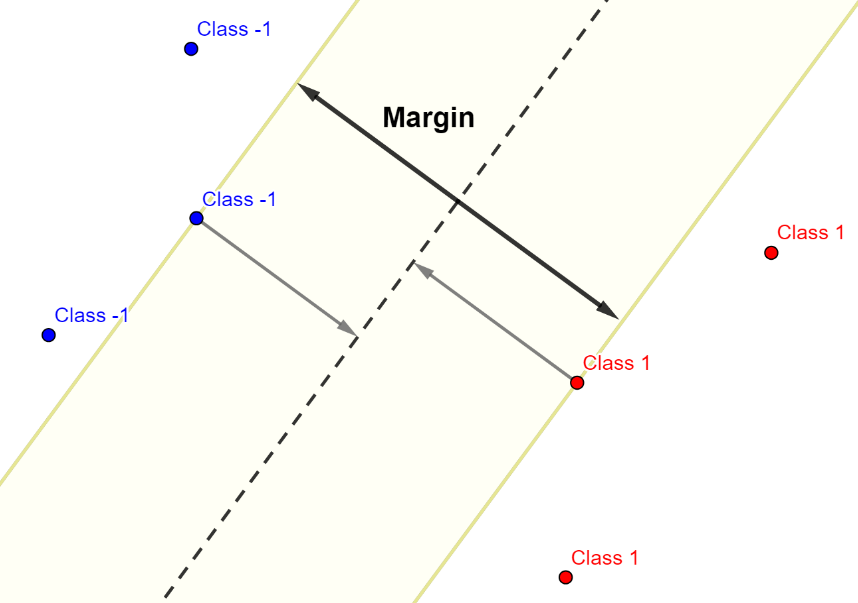
\includegraphics[width=0.7\textwidth]{SVM.png}
\captionof{figure}{Figure showing a margin (black line) between two classes of data. The variable M is shown by the grey lines.}

\end{center}

The variable M (shown as the grey lines in figure 1) is equal to half the margin distance and is the measurement of the closest point to the boundary line. The SVM algorithm finds the hyperplane that gives the maximal margin. The margin $M$ is maximised subject to the contraint
\begin{equation}
\begin{gathered}
y_i(x_i^T \beta+\beta_0)\geq M,\text{ } \forall i
\end{gathered}
\end{equation}

where $y_i$ is the target variable for a single data point $i$, formally $y_i \in \{-1, 1\}$. $\beta$ and $\beta_0$ are the coefficients of the hyperplane where $M=\frac{1}{||\beta||}$. In the case where the data is not linearly separable, some points are allowed to be on the wrong side of the margin. These points are then given a slack variable $\varepsilon_i$ measured as the distance inside the margin, and new constraints are formulated:

\begin{equation}
\begin{gathered}
y_i(x_i^T \beta+\beta_0)\geq M(1-\varepsilon_i),\text{ } \forall i
\\
\sum_{i=1}^m\varepsilon_i = \text{constant}
\end{gathered}
\end{equation}

Depending on the dimensionality of the vector space of the data, and the type of “kernel” used, the geometry of the decision boundary varies. For a linear kernel the decision boundary will be a hyperplane, in 2D this is a straight line. 
\newline

The kernel trick is used to find non-linear boundaries by using a transformation to add a dimension to the feature space, and then find a hyperplane in a new feature space. The kernel describes the type of function used to create the transformation to form another dimension. A good example of how the kernel trick works would be using a tranformation (on a 2D feature space) of the form $z=x^2+y^2$ to classify a circular decision boundary centered at 0. A 2-plane would then be found parallel to the $xy$-plane at some constant $z$ value, and would translate to a circular decision boundary.
\newline

When an SVM is used to classify more than two classes, there has to be some reduction of the problem to make is binary. Often what is used is a "One-Vs-Rest" strategy, in which a class is treated as normal but the remaining classes are combined together.

\subsection{Neural Network}

A neural network is a machine learning technique that can be used for classifying data. The theory of computational neural networks was originally formulated in 1943 [McCulloch, Warren; Walter Pitts (1943). "A Logical Calculus of Ideas Immanent in Nervous Activity], however, due to the computational power needed, models were not commonly used until later on in the 20th century.  
\newline
\newline
Neural networks are constructed with layers of nodes with directed links between nodes in subsequent layers as seen in Figure 2. the first layer has a node for each input dimension or feature, whereas the last layer has a node for each possible output class or label. Between the first and last layers there can be a number of hidden layers, with the number of nodes in each layer being varied depending on the complexity of the model. Every layer excluding the output layer will have a bias node that will always be active (i.e. have a value of 1). The reason for the bias node is obvious if you consider the input $x=0$ and $y=0$, because without the bias node, the outputs would all be 0. Each node from the input layer is connected to all the nodes in the subsequent layer with a forward directed and weighted link. This structure repeats in the same manner to the final output layer. 

\begin{center}
\includegraphics[width=0.7\textwidth]{NN.png}
\captionof{figure}{Figure showing a simple neural network. The network contains two input nodes, one hidden layer containing a bias node and two other hidden layer nodes, and an output layer with two output nodes.}

\end{center}

To compute the activation $z$ of a node $j$ in layer $l$, the input nodes are multiplied by their relative weights and all summed
\begin{equation}
z^{(l)}_j = \sum_{i=1}^N \theta_i a^{(l-1)}_i
\end{equation}

where $N$ is the number of nodes that have links connected towards node $j$. The value of this sum is then inputted into an “activation function” that will return a value between 0 and 1. One example of an activation function commonly used is the sigmoid function, 

\begin{equation}
h(z)=\frac{1}{1+e^{-z}}
\end{equation}

To train a neural network, the weights are randomly initialised and a training sample is inputted at the first layer of nodes. The values are then fed-forward through the network to give a reading at each output node between 0 and 1, which can be heuristically interpreted in a trained model as the probability that the input is in a given class. 
\newline

At this point, the outputted values are compared to the data points given layer and the “error” of the predicted output is inputted into a cost function. A cost function that is commonly used is the square mean loss, given by
\begin{equation}
J(\theta) = \frac{1}{2m}\sum_{i=1}^m ||y_i-h(z^{output}_i)||^2
\end{equation}
where $y_i$ is the target output vector for data point $i$ with $m$ training samples.
\newline

To train the neural network, the weights are altered so that the cost function is minimised.  This is known as backpropagation. Using the derivative of the cost function, The weights are adjusted by using an optimisation method, for example, gradient descent to minimise the cost as a function of the weights. For this method we want to see how the cost $J$ changes with respect to a change in the weight $\theta$, this is given by
\begin{equation}
\frac{\partial J}{\partial \theta} = \frac{\partial J}{\partial h} \frac{\partial h}{\partial z} \frac{\partial z}{\partial \theta}
\end{equation}
where $h$ is the sigmoid function, and $z$ is the activation of a node. This can be calculated for every weight in the network, and by applying a gradient descent algorithm, the weights are altered for each training sample. For the earlier layers in the network, the network can be followed backwards with the cost term giving an error for a specific activation node, the same method of using a gradient descent is then used at the node.

\subsection{Decision Tree}

A decision tree classifier works by using simple decision rules to identify the class of some inputted data. The feature space is partitioned repeatedly through these decision rules until the classes are grouped together. 

\begin{figure}[h]
    \centering
    \subfloat[The decision boundary produced by the decision tree graph (b)]{{\includegraphics[width=7cm]{DT.png} }}%
    \qquad
    \subfloat[The decision tree graph for inputs $x$ and $y$]{{\includegraphics[width=7cm]{DT2.png} }}%
    \caption{Figure showing the decision tree graph (b) and respective boundary (a).}%
    \label{fig:example}%
\end{figure}

The rules used to partition the space are chosen by computing the Gini impurity, which is calculated for a set of points with $J$ classes by
\begin{equation}
I_{Gini}(p, J)=1-\sum_{i=1}^Jp_i^2
\end{equation}

where $p_i$ is the fraction of items in class $i$. Gini inpurity is a measure of how mixed a subset of elements from the various classes are. To choose a rule, consider a parent set of $N$ points containing $J$ classes, and a rule that produces two child branches containing $J_0$ classes with $N_0$ data points, and $J_1$ classes with $N_1$ data points. We then measure the information gain $IG$ by looking at the parent Gini impurity, and the Gini impurity of the two child branches, and take the weighted mean

\begin{equation}
IG= N\cdot I_{Gini}(p, J) - (N_0\cdot I_{Gini}(p, J_0) + N_1\cdot I_{Gini}(p, J_1))
\end{equation}

Information gain is then measured for all possible splits, and the split/rule that gives the highest information gain is chosen. This process is then recursively made until either a chosen $max\ depth$ is reached or all training data has been separated.  

\newpage
\section{Optimisation}

When trying to find a 2D projection of the data that maximises the accuracy of a machine learning model, it is generally not efficient to use the Grand Tour algorithm. Instead, new rotation matrices should be constructed without the use of the Grand Tour algorithm. This is because the Grand Tour's purpose is to give a sequence of rotation matrices that can be combined to create a smooth animation of the data from as many angles as possible. By constructing rotation matrices without the constraints of the Grand Tour, the time to find local and global maxima is decreased.

\subsection{Mathematical Structure}

Each rotation matrix $\bm{A}$ applied to a dataset, will have a corresponding value for an accuracy measure. In an $n$-dimensional feature space, all $n\times n$ rotation matrices will need to be elements of the special orthogonal group $SO(n)$. Therefore, new rotation matrices that are created will need a determinant of +1. This requirement puts constraints on the elements in the matrices:
\begin{equation}
\sum_{k}A_{ik}A_{jk} = \delta_{ij}
\end{equation}

where $A_{ij}$ represents the element in the $i^{th}$ row and $j^{th}$ column of the rotation matrix $\bm{A}$, and $\delta_{ij}$ is the Kronecker delta. 
\newline

Consider the transformation equation given by equation (2), given that the projection wanted is 2D, only two rows of the rotation matrix need to be quantified. To simplify the problem the following vectors are used: 
\begin{align}
\bm{a}_1 = \begin{bmatrix}
           A_{11} \\
           A_{12} \\
           \vdots \\
           A_{1n}
           \end{bmatrix} 
           && 
\bm{a}_2 = \begin{bmatrix}
           A_{21} \\
           A_{22} \\
           \vdots \\
           A_{2n}
           \end{bmatrix}
\end{align} 

The constraints given by equation (13) can now be re-written as
\begin{equation}
\begin{split}
\bm{a}_1 \cdot \bm{a}_1 = 1 
\\
\bm{a}_2 \cdot \bm{a}_2 = 1
\end{split}
\end{equation}
\begin{equation}
\bm{a}_1 \cdot \bm{a}_2 = 0
\end{equation}

Using the contraints from equation (15), $\bm{a}_1$ and $\bm{a}_2$ can be considered as vectors pointing to the edge of an $(n-1)$-sphere in the vector space $\mathbb{R}^n$. From the constraint given by equation (16) the two vectors are required to be orthogonal to each other as shown in Figure 4. 
\begin{center}
\includegraphics[width=0.6\textwidth]{OrthogV.png}
\captionof{figure}{Figure showing the $n=3$ case with a sphere. The second horizontal vector can point anywhere on the dotted "equator" line to satisfy the orthogonality condition.}

\end{center}

Due to the vectors being contained on a $n$-sphere (from equation (15)), it is natural to transform the elements of the vectors into $n$-dimensional spherical polar coordinates. 
\begin{align}
\bm{a} = \begin{bmatrix}
           \cos(\theta_1) \\
           \sin(\theta_1)\cos(\theta_2) \\
           \sin(\theta_1)\sin(\theta_2)\cos(\theta_3) \\
           \vdots \\
		   \sin(\theta_1) \dotsc \sin(\theta_{n-2})\cos(\theta_{n-1}) \\
           \sin(\theta_1) \dotsc \sin(\theta_{n-2})\sin(\theta_{n-1})
           \end{bmatrix}
\end{align}

where $\theta_1 \in [0,\ \pi]$ and $\theta_i \in [0,\ 2\pi]$ $\forall \ i > 1$. 

\subsection{Finding an Optimum Projection}

To fufill the orthogonality constraint, two intial vectors are set to

\begin{align}
\bm{a}_1^{\prime} = \begin{bmatrix}
           \ 1 \ \\
           0 \\
           \vdots \\
           0
           \end{bmatrix} 
           && 
\bm{a}_2^{\prime} = \begin{bmatrix}
           \ 0 \ \\
           0 \\
           \vdots \\
           1
           \end{bmatrix} 
\end{align}

To optimise for machine learning accuracy, we now want a rotation $\bm{R}$ to be applied to both vectors (this ensures the orthogonality is conserved). To construct the rotation $\bm{R}$ that produces the maximum accuracy, we multiply all the rotation matrices that rotate the $i^{th}$-axis towards the $(i+1)^{th}$-axis in the form
\begin{equation}
\bm{R}=\bm{O}_{n-1} \times \bm{O}_{n-2} \times \dotsc \times \bm{O}_{1} 
\end{equation}
where $\bm{O}_{i}$ is defined by
\begin{equation}
\bm{O}_i(\phi_i) = 
\begin{pmatrix}
  1 &  \cdots & 0 & 0 & \cdots &  0 \\
  \vdots  &  \ddots & \vdots& \vdots & &\vdots  \\
  0 & \cdots & \cos{\phi_i} & -\sin{\phi_i} &  \cdots & 0 \\
  0 &  \cdots & \sin{\phi_i} & \cos{\phi_i} &  \cdots & 0 \\
  \vdots  &  \ & \vdots& \vdots &\ddots&\vdots  \\
  0 & \cdots & 0 & 0 & \cdots & 1
 \end{pmatrix}.
\end{equation}

The starting values for the angles used in the rotation matrices $\phi_i=\frac{\pi}{2}$ where $i=1,\dotsc,n-2$, and $\phi_{n-1}$ is varied between $[0, 2\pi]$ by dividing the interval into equal parts. The values taken by $\phi_{n-1}$ are each used to generate $\bm{R}$ in equation (19) and then transformed by transformation equations
\begin{equation}
\begin{split}
\bm{R} \bm{a}_1^{\prime} = \bm{a}_1
\\
\bm{R} \bm{a}_2^{\prime} = \bm{a}_2
\end{split}
\end{equation}
giving the first two rows of the transformation matrix used on the data to perform a projection. The new $x^{\prime}$ and $y^{\prime}$ values that the machine learning trains a model on is then given by
\begin{equation}
\begin{split}
x^{\prime}=\bm{a}_1^T \ \bm{x}
\\
y^{\prime}=\bm{a}_2^T \ \bm{x}
\end{split}
\end{equation}
where $\bm{x}$ is a data point in $n$-dimensional feature space and $\bm{a}_i^T$ represents the transpose of $\bm{a}_i$. The machine learning accuracy is then evaluated in each of the new 2D spaces. Whichever value for $\phi_{n-1}$ returns the best accuracy is kept. The process is then repeated for $\phi_{n-2}$ while keeping $\phi_{n-1}$ the same. When this step has been repeated for every value of $\phi_i$ (while keeping all $\phi_{j}$ the same, where $j>i$) we have now fully quantified $\bm{a}_1$. It is also true that each angle $\phi_i$ used in equations (19) and (20) are the spherical polar angles for $\bm{a}_1$ in the form shown in equation (17).
\newline

To optimise $\bm{a}_2$, we now alter each of the angles of the spherical polar coordinates excluding $\theta_1$ which is set to $\frac{\pi}{2}$ to ensure orthogonality. As with the $\phi_i$ angles, the angle $\theta_{n-1}$ is altered first by testing different values uniformly between $[0, 2\pi]$. With each of these values for $\bm{a}_2^{\prime}$ the transformations in equation (21) and equation (22) are used to produce a 2D space to find the accuracy measure given by the machine learning model. Whichever angle produces the highest accuracy is kept, and the next angle in descending order is now altered. This is repeated until every angle has been optimised.
\newline

After these steps, an optimum projection has been found.
\newpage
\section{Results}

After producing the Grand Tour projections for a data-set, the machine learning algorithms were applied at each time-step to give a sense of how "useful" a projection is. For the most part, the algorithm was applied to 1000 iterations of the Grand Tour.
\subsection{Machine Learning Performance on the Grand Tour}

The Grand Tour was performed for 1000 iterations. At each iteration, the three machine learning models were trained on the $x$ and $y$ values. The accuracy for each model was then found. An example of how the machine learning model accuracy varied over the Grand Tour is given below for the room data-set.
\begin{center}
\includegraphics[width=1.01\textwidth]{room_graph1.png}
\captionof{figure}{Figure showing the graph of relative performances of the machine learning techniques over the room data-set.}

\end{center}


A comparison of all the machine learning model's performances is given in the table below for all the data-sets.

\begin{table}[h]
\caption{Table showing the machine learning performances of the data-sets used. Measure A is the maximum accuracy found in the 1000 iterations on the Grand Tour. Measure B is the number of iterations where that machine learning model performed better than the other two.}
\begin{tabular}{r|c|c|c|c|c|c|c|c|c|c|c|c|} 
\cline{2-13}

\multicolumn{1}{l|}{}              & \multicolumn{12}{c|}{\textbf{Dataset}}                                                                                                                                      \\ \cline{2-13} 
\multicolumn{1}{l|}{}              & \multicolumn{2}{c|}{Room} & \multicolumn{2}{c|}{Particle} & \multicolumn{2}{c|}{Bank} & \multicolumn{2}{c|}{Blood} & \multicolumn{2}{c|}{Spine} & \multicolumn{2}{c|}{Iris} \\ \cline{2-13} 
                                   & A             & B         & A               & B           & A             & B         & A              & B         & A              & B         & A            & B          \\ \hline
\multicolumn{1}{|r|}{\textbf{SVM}} & 99.42\%       & 145       & 85.05\%         & 26          & 99.34\%       & 265       & 77.51\%        & 0         & 75.73\%        & 81        & 96\%         & 15         \\ \hline
\multicolumn{1}{|r|}{\textbf{NN}}  & 99.42\%       & 472       & 86.19\%         & 152         & 100\%         & 529       & 81.52\%        & 637       & 80.58\%        & 329       & 98\%         & 534        \\ \hline
\multicolumn{1}{|r|}{\textbf{DT}}  & 99.32\%       & 319       & 90.76\%         & 266         & 98.91\%       & 138       & 81.52\%        & 180       & 80.58\%        & 469       & 98\%         & 192        \\ \hline

\end{tabular}

\end{table}




\newpage
\subsection{Optimisation Performance}
\newpage
\section{Conclusion}

Using the grand tour for data mining has some interesting properties. Some insight into dimensionality reduction can be made by finding the projections that maximise the various machine learning algorithms. Looking at the relevant rotation matrices, how much of each feature or dimension appears in the new convoluted basis vectors gives insight to which features are important in distinguishing for a certain class.
\newline
\newline
One suggestion was to look into if the Hilbert curve could be used to look at the data from many different unique projections, as it uniformly covers the space. This was not pursued as there is a problem in defining the projection. In 3D, a vector from a Hilbert curve node to the centre of the data uniquely defines a plane. This is because the vector can be used to restrict one dimension and use two orthogonal unit vectors to create a basis for a subspace. However, when the feature space exceeds three dimensions there is a problem with this method. In a 4D feature space, two unique vectors are needed to define a unique plane. After using the vector defined from the Hilbert node to the centre of feature space, the subspace still needs to be reduced by one dimension to get a 2D space. 
\newline
\newline
Something that would be interesting to investigate further is to see if a new unsupervised learning clustering algorithm could be developed to group data into classes. By looking at how much each data point moves relative to another data point in the tour (travel matrix), could this give insight to classification groupings? After looking at the matrix colourmap of this variable, three rectangular shaped structures can be seen in the ordered data. By using network community detection algorithms or some other clustering analysis, would this method work, and more importantly, how would it compare to current unsupervised learning algorithms as the travel matrix is somewhat similar to the distance between points in the feature space.

\bibliography{test}

\end{document}
